\chapter{Knowledge Ports}
\label{sec:knowledgePorts}
We have learned a lot about vocabulary and knowledge. Now, we can discuss communication. {\it Entities} communicate in each distributed system. Client-Server systems define two classes of {\it entities}. Clients communicate with servers. Each entity has its designated role in each communication act. They can change roles, though. A computer that is server in one communication can be client in another one.

Shark based applications are P2P applications. Each Shark peer should be aware of receiving messages. Each Shark peer can send anytime any other peer a message. Shark communication paradigm can be compared with a crowded party. People who might never seen before exchange some words and go away. Maybe they see again, maybe not. People can say something. Maybe it is understood or not.
People can also exchange phone numbers and addresses. After that, they can talk even if they are no longer at this party. 

That's the very idea of Shark. Peers can communicate whenever they want to but they have no obligation to answer in a defined manner. Shark makes no constraints about communication behavior. It's up to the application.

A leaflet application might deliver an advertisement to any peer. Certainly, it won't be seen as {\it rude} if peers don't react. A leaflet sender can not assume a {\it thank you} or whatever.

Another application might be a decentralized social network\footnote{SharkNet is
a growing example. It actually is a social network based on Shark, see our web page for project status.}. In such application it can be helpful to know if information has received its destination or not. Such handshakes can be coded by applications programs. We'll see an example in section \ref{sec:chatkp}.

Communication requires a protocol. This protocol is called {\it Knowledge Exchange Protocol (KEP)}. It has just two commands: 

\begin{description}
    \item[Expose] sends an interest to a peer.
    \item[Insert] sends knowledge to a peer.
\end{description}

Application logic can be implemented with {\it Knowledge Ports} in Shark which are sometime called {\it Sharklets}. It is a quite slim interfaces. 

Creating your own application specific knowledge port is simple as to be seen in the following code:

\begin{verbatim}
public class MyKP extends KnowledgePort {
   public MyKP(SharkEngine se) {
      super(se);
   }

   @Override
   protected void doInsert(Knowledge knowledge, 
                           KEPConnection kepConnection) {

      // do something useful here - or not
   }

   @Override
   protected void doExpose(SharkCS interest, 
                           KEPConnection kepConnection) {

      // do something useful here - or not
   }
}
\end{verbatim}

We will discuss the KEP protocol itself very briefly in this chapter. Shark creates messages which are sent over the network.

This chapter discusses how to write your own knowledge port. Shark has some predefined knowledge port. They will be presented. The most important is our {\tt StandardKP}. We claim, that most applications can be implemented with it by setting appropriate parameters. 

\section{Implementing your own Knowledge Port}
Each knowledge port must be derived from {\tt KnowledgePort}. Each knowledge port must run with a {\tt SharkEngine}, see next chapter. Thus, each knowledge port {\it must} call the constructor that sets this engine.

\begin{verbatim}
public class MyKP extends KnowledgePort {
   public MyKP(SharkEngine se) {
      super(se);
   }

//...
\end{verbatim}

{\tt KnowledgePort} is abstract because two methods are abstract which have to be implemented by non-abstract knowledge ports.


\begin{verbatim}
   @Override
   protected void doInsert(Knowledge knowledge, 
                           KEPConnection kepConnection) {
      // do something useful here - or not
   }

   @Override
   protected void doExpose(SharkCS interest, 
                           KEPConnection kepConnection) {
      // do something useful here - or not
   }
}
\end{verbatim}

Abstract class {\tt KnowledgePort} offers a number of useful methods which are explained throughout that section and can also be found in the online API description\footnote{http://sharkfw.sourceforge.net/api/current/net/sharkfw/peer/KnowledgePort.html}.

\subsection{KEPConnection}
Knowledge ports are called when KEP message reaches a peer. They have to handle either interests or knowledge. Any knowledge ports must implement two methods for that reason: {\tt doExpose} to handle interests and {\tt doInsert} to handle knowledge. 

Both methods have two parameters: First is an interest or knowledge. Second is a {\tt KEPConnection} object. We are going to explain some details of that object in this section.

{\tt KEPConnection} allows to check whether an message was encrypted and / or signed.

\begin{verbatim}
protected void doExpose(SharkCS interest, 
                  KEPConnection kepConnection) {
//...
  if( kepConnection.receivedMessageEncrypted() {
    // message was encrypted
  }
  if(kepConnection.receivedMessageSigned()) {
    // message was signed
  }
}
\end{verbatim}

\subsubsection{Reply}
Peer often want to reply to incoming interests or knowledge. A reply can be an arbitrary number of expose and insert messages. In other words, a peer can reply with interests and knowledge. 

A reply is sent by means of the {\tt KEPConnection} object by calling {\tt expose} or {\tt insert} with appropriate parameters.

There are a three variants of {\tt expose}. Have a look at the following code fragment.

\begin{verbatim}
Interest i = // create an interest
try {
 kepConnection.expose(i);
} catch (SharkException ex) {
 // do something 
}
}
\end{verbatim}

The actual interest is less important for this example. We just need one. Now, {\tt kepConnection} is used to send this interest to the peer from whom we have received the KEP message in the first place. In short: It is a direct reply. An exception can be thrown if something went wrong during delivery.

There is another variant:

\begin{verbatim}
String address = "mail://alice@wonderland.gov";
try {
   kepConnection.expose(interest, address);
} catch (SharkException ex) {
   // do something
}
\end{verbatim}

The reply is sent to a dedicated address instead to the sending peer. The final variant takes an array of addresses instead a single address, see online documentation. The interest is sent to each address in the list.

The same concept is used if knowledge is to be sent as reply. Note, there is no method that sends knowledge just to the sending peer. It is for developers safety and not for their punishment.

We figured that developers tend to become confused by all those peers which can be seen as sender. Shark philosophy is that interests tend to be commonly available but knowledge not. We think, that sending knowledge must happen deliberately. Let's have a look of different kind of sender.

\subsection{Physical and logical sender}
\label{sec:knowledgePorts:sender}

\begin{figure}[t]
\centering
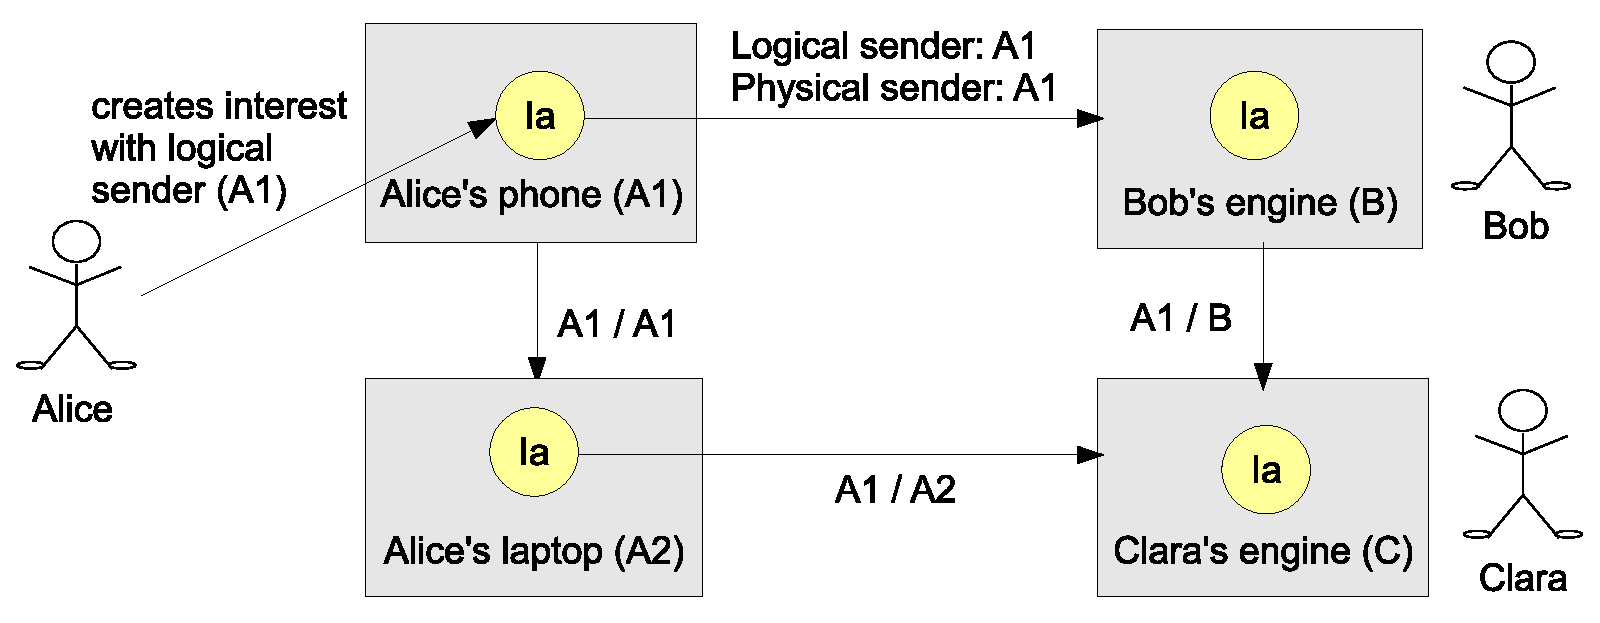
\includegraphics[width=0.80\textwidth]{physicalAndLogicalSender.eps}
\caption{Physical and logical sender}
\label{fig:physicalAndLogicalSender}
\end{figure}

Whenever a peer has received a KEP message there was a {\it physical sender} which is a computer, smartphone, etc. that issued the message. That message can be encrypted and signed. Neither of them ensures that the physical sender is actually the peer that is described in {\it peer dimension} of the interest or knowledge. That peer is called {\it logical sender}. When we talk about a {\it sender}, we already mean the {\it logical sender}.

A {\it logical sender} can create a message, can even sign and encrypt but can store it in another device which transmits this message to others. Thus, the other devices or peers can act as proxies or relays. Recipients can decide whether to reply to the proxy or directly to the {\it logical sender}. 

Figure \ref{fig:physicalAndLogicalSender} illustrates the relation between {\it logical} and {\it physical} sender. Alice creates an interest in this example. She stores that interest on her device A1. She also decided to choose A1 as logical sender. Note, each peer, each user is free to define a logical sender address. We have already defined an number of addresses for peers throughout that book. All addresses in peer semantic tags are {\it logical} addresses and can freely be chosen by users.

In this example, Alice chooses A1 as logical address and stores her interest also on A1. She meets Bob and exposes her interest. In that case, physical and logical sender are identical.

Bob can forward Alice's interest (unchanged) to Clara. Alice is still logical sender but Bob's device is logical sender. 

Alice could also synchronize her data to another device, e.g. her laptop. Her interest could also be sent from her laptop to Clara. In that case, A1 is still logical but A2 is physical sender.

{\tt KEPConnection} offers several methods to reply to incoming interests. The more convenient methods reply to the {\it physical} sender. In most cases, this would be an appropriate choice but not in any. 

Moreover, information of physical sender are not stored in interests or knowledge. That information is only available when receiving that data.
Applications who need physical sender information are required to save it.
Physical sender address can be retrieve from the connection object.

\begin{verbatim}
PeerSemanticTag sender = kepConnection.getSender();
String[] addresses = sender.getAddresses();
\end{verbatim}

We encourage to defines recipient addresses explicitly. That makes your code more transparent for other programmers.

Shark allows signing and encrypting. Shark only offers End-to-End-Encryption. Physical sender don't play any role in those scenarios. Logical sender sign and encrypt. Physical devices are only means for transportation.

\subsection{Sending initial messages}
It isn't enough to wait for incoming requests. One peer must start talking.

{\tt KnowledgePort} objects support methods for sending interests and knowledge. The following code is a sketch of its usage.

\begin{verbatim}
Knowledge k = ...
Interest i = ...
PeerSemanticTag peer = ...
this.sendKnowledge(k, peer);
this.sendInterest(i, peer);
\end{verbatim}

The code is straightforward. We need a peer and either knowledge or an interest which can be delivered. Sending might fail either for security reasons or network problems. Exception are thrown in either case.

A KEP message is send in case of success and be be handled by the receiver, more specific by a receivers {\tt KnowledgePort} objects. Note, message can send with each running knowledge port. The sending port has no privileges over others. A reply on a sent message is handled as any other message and offered to each active knowledge port.

Thus, sending a message requires at least a single active knowledge port. 
There are no methods (yet) that allows developers to send {\it interest} or {\it knowledge} without a {\tt KnowledgePort} object. In the rare case of a peer that has no knowledge a workaround is proposed: Implement your own knowledge port and leave {\tt doExpose} and {\tt doInsert} empty. Now you have a knowledge port that actually has no effect on incoming messages but can be used to send messages.

\subsection{Creating a knowledge port}
Now we are ready to instantiate a knowledge port. We need a {\tt SharkEngine} first, see chapter \ref{sec:sharkengine} for details. Afterwards, we can bring our knowledge port into existence and action:

\begin{verbatim}
SharkEngine se = new J2SEAndroidSharkEngine();
KnowledgePort kp = new MyKP(se);
\end{verbatim}

The port is up and running now. Knowledge port management is discussed in the {\tt SharkEngine} chapter.

\subsection{KP Listener}
{\tt KnowledgePort} objects can be observed. The following code implements a class that listens to knowledge port activities.

\begin{verbatim}
public class MyKPListener implements KPListener {
  public void exposeSent(KnowledgePort kp, 
                         SharkCS sentMutualInterest) {
    System.out.println("expose received");
  }

  public void insertSent(KnowledgePort kp, 
                         Knowledge sentKnowledge) {
    System.out.println("insert received");
  }

  public void knowledgeAssimilated(KnowledgePort kp, 
                                   ContextPoint newCP) {
    System.out.println("KP has assimilated something");
  }
}
\end{verbatim}

This class implements the {\tt KPListener} interface that comprises three methods which are implemented in a quite naive way.

A listener must be added to a knowledge port. Let's extend our example code from previous section:

\begin{verbatim}
SharkEngine se = new J2SEAndroidSharkEngine();
KnowledgePort kp = new MyKP(se);
KPListener myListener = new MyKPListener();
kp.addListener(myListener);
\end{verbatim}

{\bf Knowledge port developer have to trigger those listener events!} The {\tt KnowledgePort} class just offers methods to subscribe and remove listeners.
It does {\it not} trigger e.g. a {\tt exposeSent} event. This is up to knowledge port developers!

Triggering those events is very simple, though. The following code can be  called inside any knowledge port object.

\begin{verbatim}
// get or create interest and send it
Interest i = ...
// notify listeners that an interest was exposed
this.notifyExposeSent(this, i);

// create or get knowledge and send it
Knowledge k = ...
// notify listener about send knowledge
this.notifyInsertSent(KnowledgePort kp, k);

// get context point and write to knowledge base
ContextPoint cp = ...
// notify listeners
notifyKnowledgeAssimilated(KnowledgePort kp, cp);
\end{verbatim}

\subsection{Other methods}
Knowledge ports can be stopped and restarted again.

\begin{verbatim}
..
KnowledgePort kp = ...
kp.stop();
..
kp.start();

boolean started = kp.isStarted();
\end{verbatim}

A stopped knowledge port does not get any KEP message until it is restarted again. 

Each knowledge port can hold a knowledge base. We have added this feature into the most abstract superclass because most knowledge ports will need a knowledge base for operations.

\begin{verbatim}
..
SharkKB kb = ...
kp.setKB(kb);
..
kb = kp.getKB();
\end{verbatim}

Most knowledge ports will work with an interest. There are methods to set and get interests.

\begin{verbatim}
..
Interest i = ...
kp.setInterest(i);
..

i = kp.getInterest();

// does kp have a receiving  and/or sending interest?
boolean receivingInterest = kp.isIKP();
boolean sendingInterest = kp.isOKP();
\end{verbatim}

Lets summarize. Knowledge ports are {\it the element} that stores the actual application logic of peers. Knowledge ports work independently from each other. Thus, a peer can instantiate a number of ports that perform different tasks.

Writing a knowledge port is as difficult or as easy as writing a Servlet. 

Moreover, there are some knowledge port implementation already in the framework. We guess that this number of predefined knowledge ports will increase over the years and releases. Next section will explain the most important knowledge ports. We start with the most generic port which is called {\tt StandardKP}. It can be configured in different ways. We hope that this generic port can solve most applications needs just be configuration. Reading and understanding the following section can seriously reduce your development time. Enjoy!

\section{Exercises}

\begin{enumerate}
\item 
Create a knowledge port that... Implement your own KP.
\end{enumerate}
